
\chapter{Implementation}
First part of this chapter . Starting with its component architecture, followed by a flow diagram and at last, it tells how to extend this framework by adding message handlers and behaviour agent for both vehicle and roadside infrastructure for creating new ITS application.

\section{Framework}
    It is a ITS simulation framework written in Python to spawn vehicle and roadside ITS subsystem in Carla simulator, It takes care of creating and maintaining the life-time of the actors in the simulation and provides extensions to customise the behaviour of the actors and messages to interact with other actors. 
    
\subsection{Configuring the Framework}
A set of key-value pairs configures the framework and the spawned actor, and they are:
\begin{itemize}
    
    \item \textbf{CarlaHost: } This is a required property to provide the IP address of Carla server. 
    \item \textbf{CarlaPort: } This is a required property to provide the port of Carla server.
    \item \textbf{Port: } This is a required property to provide the port of actors socket server.
    \item \textbf{Type: } This is a required property, and based on this the framework spawns a vehicle or RSU in the Carla server. It should be either Vehicle or RSU.
    \item \textbf{CommunicationRange: } This is a required property, and based on this the communication of the actor is set.
    \item \textbf{ActorSpawning: } This is an optional property, and based on the spawn point of the actor is determined. The actor is spawned at a random location if the value is not available.
    \item \textbf{ActorDestination: } This is an optional property. Based on this the vehicle destination is decided. The destination is selected at random if the value is not available.
\end{itemize}
\subsection{Component Architecture}

\begin{figure}[h!]
    \centering
    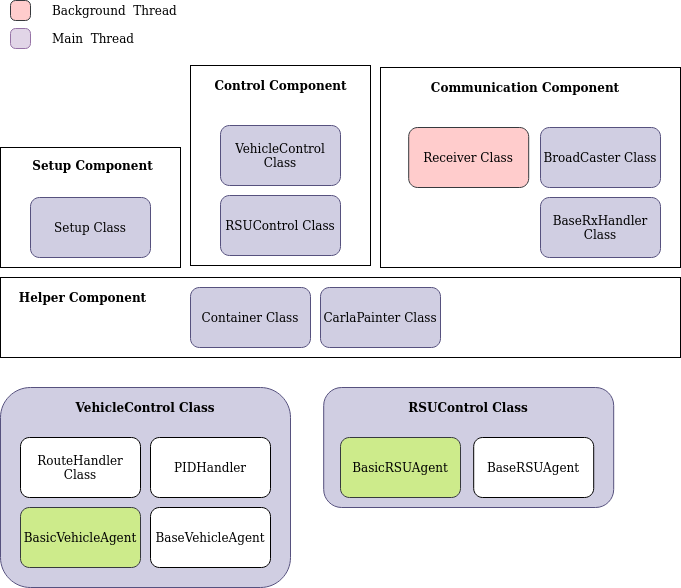
\includegraphics[width=12cm]{Framework/Images/FArc.png}.
    \caption{Component Architecture}
    \label{arrrk}
\end{figure}

The framework has four components are they are divided based on functionality. The figure \ref{arrrk} is the component architecture of the framework and the entire class diagram is available in the appendix.

\subsubsection{Setup Component}
The responsibility of this component is to set up the entire framework to spawn the actor in the Carla server. It has only one class called \say{Setup} that acts as the entry point for the framework. The code snippet in the figure \ref{init} shows how to initialise the framework.The responsibility of  \say{Setup class} is to create Carla Client instance, initialise the states and global variables. 

\begin{figure}[h!]
    \centering
    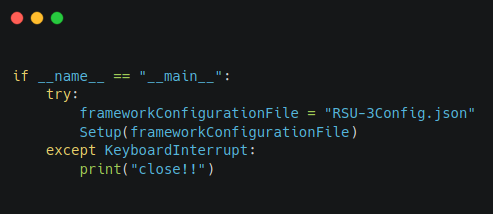
\includegraphics[width=10cm]{Framework/Images/init.png}.
    \caption{Code Snippet to Initialise The Framework}
    \label{init}
\end{figure}

\subsubsection{Control Component}
This component is responsible for creating, spawning and maintaining the lifetime and controlling the actor. This component separate control class for RSU and vehicle called \say{VehicleControl} and \say{RSUControl}. The \say{VehicleControl Class} has a driver agent that acts as the mobility model for the vehicle and the agent is based on waypoint navigation.

\subsubsection{Communication Component}
This component is responsible for broadcasting and receiving messages. It plays a vital role in establishing the coordination and cooperation between the actors. At this stage, the component only supports one-hop communication. 

The \say{Receiver class} receivers the message and pushes it to their respective message handlers based on its type. This class is responsible for initing and maintaining the lifetime of the socket server. 

The \say{BroadCaster Class} broadcasts the message to other actors within the assigned communication range. It provides V2V, V2R and V2X communication modes and based on the mode it filters the actors and sends the message to them.

\subsubsection{Helper Component}
This component provides support functioning of the framework. It has two classes, they are:

\begin{itemize}
    \item  \textbf{Container Class:} It is a singleton class that holds the states of the actor, simulation world and map throughout the life-time of the actor. Additionally, it holds the metadata of \say{Broadcaster class} and message handler classes. It also holds a key-value dictionary property to store the handled messages, and it can be retrieved by other components when needed. 
    \item \textbf{CarlaPainter Class:} It is used to create a client instance for CarlaViz and draw additional features to the visualization. It allows actors to draw text, point and lines.
\end{itemize}

\section{Extending the framework}
The framework provides extensions for certain sub-component to customize it. The decorator design pattern \cite{decorator} is used to add the customized component to the framework with affecting its behaviour. This way, users can easily customize by just creating a class and adding the decorator at the top of the class name. The rest of the explains how to add message handlers to the communication module and customise the behaviour of the vehicle and RSU.
\subsection{Vehicle Behaviour}
The behaviour of the vehicle is controlled by the driver agent of the framework. To customise, it the \say{BasicVehicleAgent class} should be overridden using the \say{@drivingAgent} decorator. 

First, a behaviour class is created inheriting from \say{BaseVehicleAgent class}. The behaviour logic is written inside the \say{RunStep} abstract function.  After creating,  the decorator is added at the top. The decorator adds the customised agent to the framework to control the vehicle behaviour.
\subsection{Roadside Infrastructure Behaviour}
The framework does not provide any behaviour agent for RSU. The behaviour agent class is added to the framework using \say{@rsuAgent} decorator. 

First, a behaviour class is created inheriting from \say{BaseRsuAgent class}. The behaviour logic is written inside the \say{RunStep} abstract function. After creating, the decorator is added at the top. The decorator adds the customised agent to the framework to control the RSU behaviour.
\subsection{Adding Message Handler}
The behaviour of actors depends on the message they receive. The framework has a collection of handlers to receive, process and stores the messages in the container class and later it can be retrieved by the agent class to compute logic based on the message. Any new message handlers can be added to the framework using \say{@addRxHandler(\say{MessageType})} decorator, where MessageType is the type of the message the class handles. (e.g., \say{@addRxHandler(\say{DENM})} for handling DENM message).

First, a handler class is created inheriting from \say{BaseRxHandler class}. The handling logic is written inside the \say{Main} abstract function. After creating, the decorator is added at the top. The decorator adds it to the handler collection in the communication module.
